\begin{figure}[!htb]
\centering

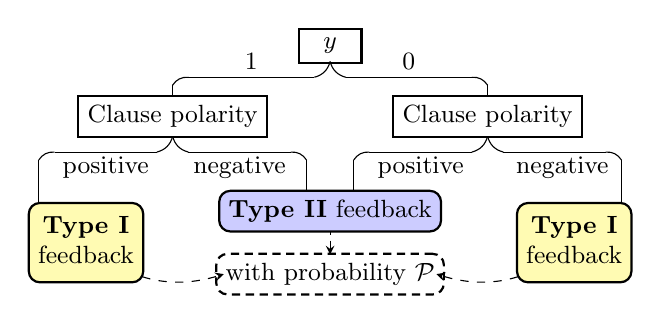
\begin{tikzpicture}[font=\small]
\node [draw, thick, shape=rectangle, minimum width=0.8cm] at (0,-0.3) {$y$};
\draw []  (0,-0.5) to [bend left] (-0.2,-0.7);
\draw [] (-0.2,-0.7) -- (-1.8,-0.7);
\node[] at (-1,-0.5) {1};
\draw []  (-1.8,-0.7) to [bend right] (-2,-0.8);
\draw [] (-2,-0.8) -- (-2,-1.25);
\draw []  (0,-0.5) to [bend right] (0.2,-0.7);
\draw [] (0.2,-0.7) -- (1.8,-0.7);
\node[] at (1,-0.5) {0};
\draw []  (1.8,-0.7) to [bend left] (2,-0.8);
\draw [] (2,-0.8) -- (2,-1.25);

\draw []  (-2,-1.45) to [bend left] (-2.2,-1.65);
\draw [] (-2.2,-1.65) -- (-3.5,-1.65);
\node[] at (-2.85,-1.85) {positive};
\draw[] (-3.5,-1.65) to [bend right] (-3.7,-1.75);
\draw[] (-3.7,-1.75) -- (-3.7,-3);
\draw []  (-2,-1.45) to [bend right] (-1.8,-1.65);
\draw [] (-1.8,-1.65) -- (-0.5,-1.65);
\node[] at (-1.15,-1.85) {negative};
\draw[] (-0.5,-1.65) to [bend left] (-0.3,-1.75);
\draw[] (-0.3,-1.75) -- (-0.3,-2.6);
\node [draw, thick, shape=rectangle, minimum width=0.8cm,fill=white] at (-2,-1.2) {Clause polarity};

\draw [-stealth,dashed]  (-3.1,-2.8) to [bend right] (-1.35,-3.2);

\node [draw, thick, shape=rectangle, minimum width=0.8cm, rounded corners, fill=yellow!30!white] at (-3.1,-2.8) {\begin{tabular}[c]{@{}c@{}} \textbf{Type I} \\ feedback \end{tabular}};

\draw []  (2,-1.45) to [bend left] (1.8,-1.65);
\draw [] (1.8,-1.65) -- (0.5,-1.65);
\node[] at (1.15,-1.85) {positive};
\draw[] (0.5,-1.65) to [bend right] (0.3,-1.75);
\draw[] (0.3,-1.75) -- (0.3,-2.6);
\draw []  (2,-1.45) to [bend right] (2.2,-1.65);
\draw [] (2.2,-1.65) -- (3.5,-1.65);
\node[] at (2.95,-1.85) {negative};
\draw[] (3.5,-1.65) to [bend left] (3.7,-1.75);
\draw[] (3.7,-1.75) -- (3.7,-2.6);
\node [draw, thick, shape=rectangle, minimum width=0.8cm,fill=white] at (2,-1.2) {Clause polarity};

\draw [-stealth, dashed]  (3.1,-2.8) to [bend left] (1.35,-3.2);

\node [draw, thick, shape=rectangle, minimum width=0.8cm, rounded corners, fill=yellow!30!white] at (3.1,-2.8) {\begin{tabular}[c]{@{}c@{}} \textbf{Type I}  \\ feedback \end{tabular}};

\draw [-stealth, densely dashed] (0,-2.6) -- (0,-2.95);

\node [draw, thick, shape=rectangle, minimum width=0.8cm, rounded corners, fill=blue!20!white] at (0,-2.4) {\textbf{Type II} feedback};

\node [draw, densely dashed, thick, shape=rectangle, minimum width=0.8cm, rounded corners] at (0,-3.2) {with probability $\mathcal{P}$};

\end{tikzpicture}

\caption{TM feedback procedure, independently performed for each clause. For binary classification, $y$=1 or 0 suggests the sample belongs to the class or not, respectively; for multiclass classification and a TM for a certain class, $y$=1 or 0 suggests the sample belongs to the class or other classes, respectively.}
\label{fig:tm_feedbacks}

\Description[overall TM feedback]

\end{figure}
